The Server Side Application (SSA) is the module responsible for creating a solution 
to a user selected request. In this case, the SSA receives a shallow Flying Tourist Problem,
that is, an instance of the problem which does not yet have the set of arcs $A$ associated to the problem.
Thus, the SSA has two main goals:

\begin{enumerate}
  \item create the list of arcs associated to the problem;
  \item produce a solution to the user selected request;
\end{enumerate}

The system which is responsible for producing the list of arcs will be denoted as \textit{Data Management System},

while the production of a solution to the user request relies on a system called \textit{Optimization System}.


\todo{Explain that the SSA consists in a way of translating user requests to FTP instances, which are than solved by the optimization algorithm previously deviced. Explain that, due to the multiple objectives of the system, we construct multiple cost matrixes for each objective function.}


\subsubsection{Data Management System}
\label{sec:dms_design}
% Data Management System

Upon receiving a user specified request, the set of nodes, aswell as the start time and durations,
are well defined. On the other hand, the set of arcs which connects these nodes is not.
For example, a user request may correspond to a single flight between $A$ and $B$ at time $t$,
and upon receiving this request, there is no information available about the flights (arcs)
which connect these two cities. In fact, thats exactly what the user is looking for.
Thus, the goal of the Data Management System is to collect the necessary information 
to construct the list of arcs associated to a user request.

It is important to note that an arc connecting two nodes corresponds 
to a flight between two cities, at a specific date. However, there are multiple 
flights which fit this discription, and every one of these flights has several attributes 
which differentiate themselves. For exemply, every flight has a particular cost,
flight duration, departure and arrival time, airline, bag limit or even 
layover flights.

Due to the vaste attributes which define every flight,
it is impossible to known which particular flight is the most adequate to a specific user,
because users often have different selection criteria.
Due to this, upon the construction of the multipartite graph,
it makes sense to have a list of possible flights, for every arc in $A$,
instead of just one.
This enables the selection of a specific flight according to the objective function being minimized.
For example, if the goal is to minimize the total fligh cost,
it makes sense to select those flights which present the lowest cost, 
disregarding other attributes of the flights as, for example, the flights duration.
This means that when talking about an arc connecting two nodes, it makes more sense to talk about 
a \textit{family} of arcs, which share key characteristics, as the origin, destination and date,
but which may vary regarding the other attributes, as flight cost and duration.


Following the definition of the Flying Tourist Problem, and the notation proposed by J.C.Picard,
a request may be defined as a multipartite graph, divided into $k$ layers,
and where every node in a layer is fully connected to every other node in the subsequent layer.
The total number of layers, which correspond to time span between the earliest date in which the trip might start,
and latest date in which it might finish, is given by equation \ref{eq:k_number_layers}.
The arcs which connect those nodes are divided into three groups: \textit{initial}, \textit{transition} and \textit{final} arcs.
Figure \ref{fig:multipartite_times} illustrates the time periods associated to each arc type,
according to the Flying Tourist Problem definition, with a multiple time start period,
and a non empty list of cities to be visited.


\begin{figure}[htpb]
  \centering
  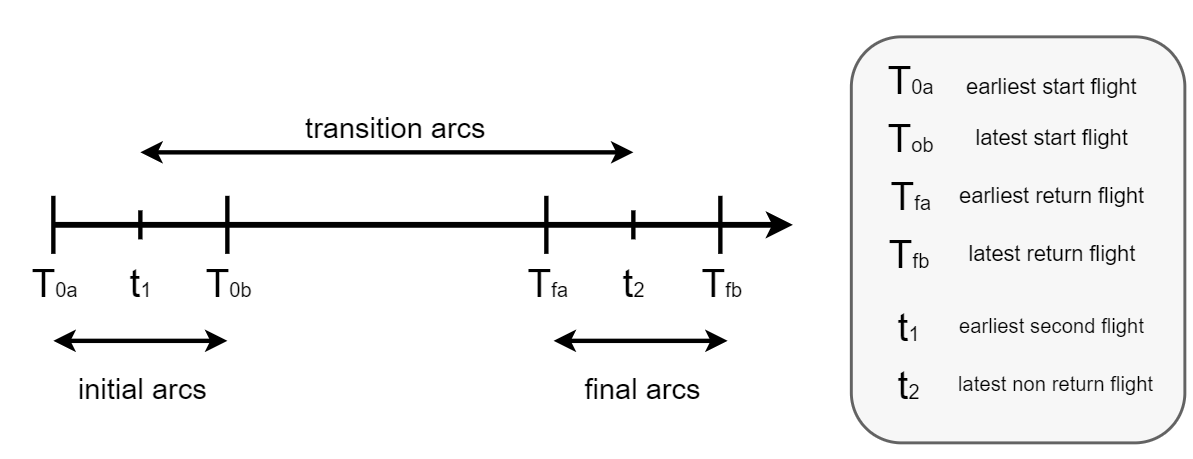
\includegraphics[width=\textwidth]{./Figures/system_design/flights_times.png}
  \caption{Illustration of the distribution in time of the initial, final and transition arcs.}
  \label{fig:multipartite_times}  
\end{figure}


\begin{equation}
\label{eq:k_number_layers}
  k = T_{fb} - T_{0a} + 1 = t_s + summ(D) + 1
\end{equation}

The initial arcs correspond to those who might initiate the trip,
and thus must start at city $v_0$ at a time $t \in T_0 = [T_{0m}, T_{0M}]$
and visit every city in $V \cup {v_{n+1}}$.
There are a total of $k_1 = T_{0M} - T_{0m} + 1 = t_s + 1$ layers for the initial arcs.

In its turn, the transition arcs are those which connect the $N$ cities 
of the list of cities to be visited $V$.
The earliest transition arc occurs at a time no sooner than $t_1 = T_{0a} + min(D)$,
where $min(D)$ corresponds to the lowest entry of the set of durations.
That is, if the trip starts at time $T_{0a}$, which is the earliest start date,
and if the minimum duration associatedto a city is $min(D)$, 
than the second flight might occur at a time no sooner than $t_1 = T_{0a} + min(D)$.
Following a similar approach, the latest transition flight can 
occur no latter than $t_2 = T_{0b} + summ(D) - min(D)$, where $summ(D)$ corresponds 
to the summ of all entries belonging to $D$.
Thus, there are a total of $k_2 = t_2-t_1+1$ transition layers.

On the other hand, the final arcs are those which might conclude the trip,
and thus must return to city $v_{n+1}$,
from a city in $V \cup \{v_0\}$. The final layer extends from 
$T_{fa}$ to $T_{fb}$, where $T_{fa}$ = $T_{0a} + summ(D)$ and $T_{fb}$ = $T_{0b} + summ(D)$.
There are a total of $k_3 = T_{fb} - T_{fa} + 1 = t_s + 1 $ final layers.
Comparing to the number of initial layers, one can conclude that there are as many 
initial layers, as there are final layers. 

In conclusion, the goal of the Data Management System is to enable the construction 
of the lists of flights which are necessary to proccess some user request.
By now, it should be clear which particular set of flights are necessary.
However, nothing was yet said about how to actually obtain the required information.

To have access to real flight data, the most simplest and efficient way is to 
find a publicly available flight data API. There are several choices regarding to this,
and it was a subject of a lot of research.
In summary, the available API's are classified as \textit{free}, \textit{limited} and \textit{unacessible}.
A free API is one which charges no charge for any query, nor limits the number of daily queries.
On the other hand, a limited API is one which sets an upper bound on the number of daily available queries,
and charges a fee after this limited. In its turn, an unacessible API is an API which is available 
only for commercial solutions, and which was unavailable to be used in a research context.
In this work, only free API's were tested and used.
The communication to an API relies on simple HTTP protocol, where the requested resource 
is specified according to a URL syntex defined by the source,
and whose response is usually in the format of JSON, corresponding to a list of flights,
with a lot of details about the attributes of each flight.
Figure \ref{fig:kiwi_response} illustrates the response of a particular API (Kiwi) to a specific query.
In this image it can be seen that there are a total of 134 flights satisfying the query (data [113]),
and that each flight has multiple attributes, as the price, duration, country etc.

\begin{figure}[htpb]
  \centering
  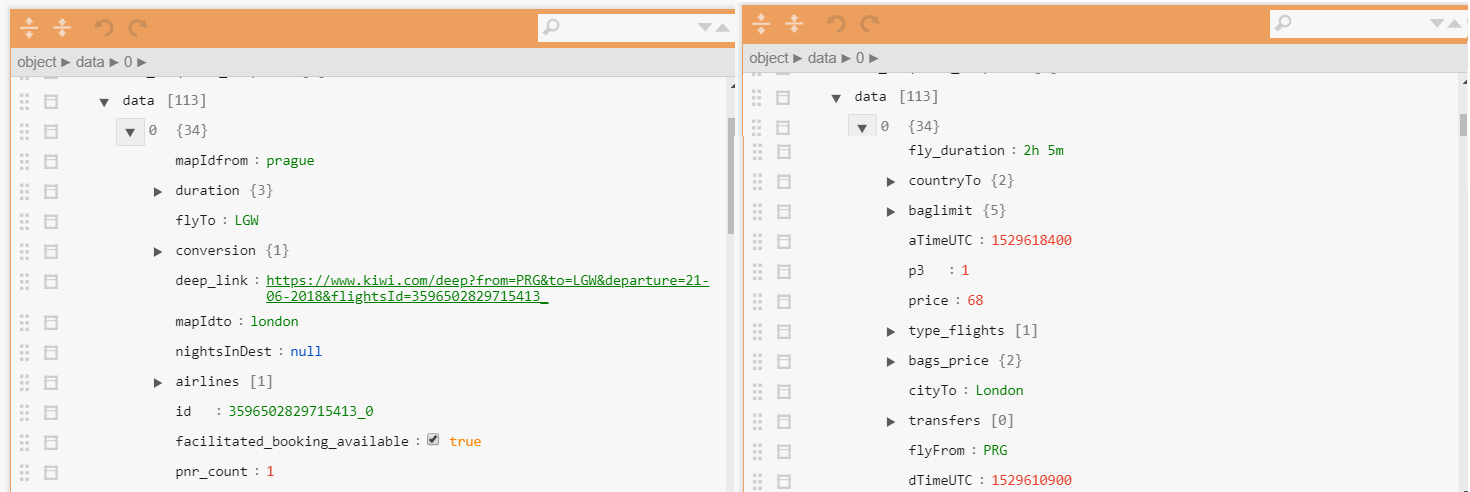
\includegraphics[width=\textwidth]{./Figures/system_design/kiwi_response.png}
  \caption{Response of Kiwi's flight API to a particular query. It can be seen 
  that multiple flights are returned, each with its own attributes.}
  \label{fig:kiwi_response}  
\end{figure}

One of the most important conclusions of testing different API's,
is that different API's provide very different results.
These results are presented in annex \textbf{anexo preços aqui!},
and show that for the same query,
flight prices may vary up to 103\%, depending on the source used.

To tackle this problem, a secondary approach was taken. Instead of using 
public API's to access real flight data, it is possible to create a program known as \textit{web scraper},
which visits a specific website in order to retrieve the information from it.
This enables the consultation of flight sources, which otherwise could not be acessed.
While webscraping has the advantage of accessing content that otherwise could not be,
it has many disadvantages. Comparing to API's,
web scraping is a lot slower, and much more difficult to actually implemenet.
Figure \ref{fig:scraping_example} illustrates the process of inherint to web scraping.
On the left is an image of a website query and results,
while on the right is the corresponding (simplified) source code.
The annotations provided identify the different flight attributes, and the locations in which they occur in the HTML code.
 
\begin{figure}[htpb]
  \centering
  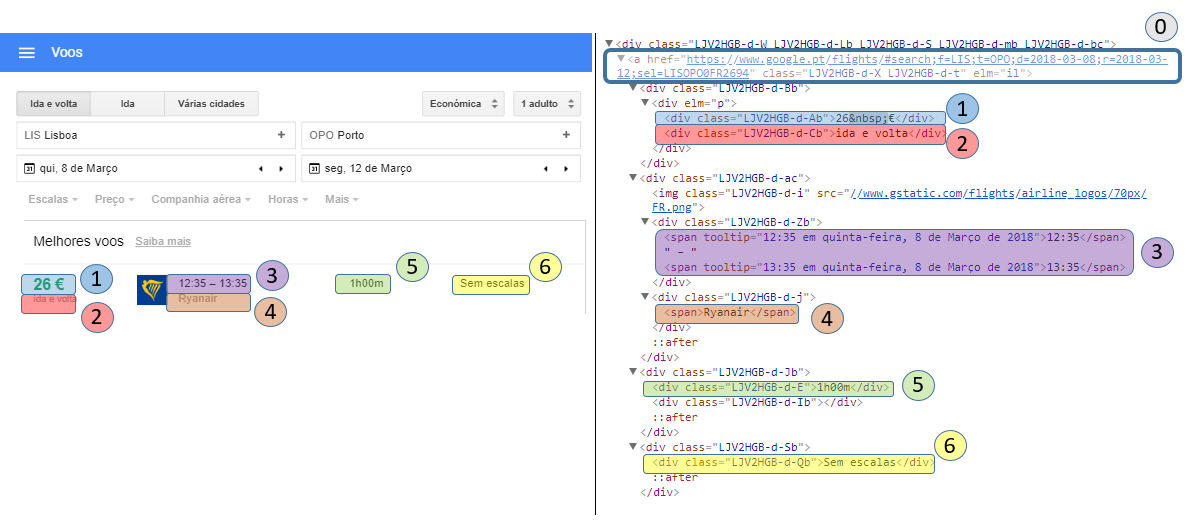
\includegraphics[width=\textwidth]{./Figures/system_design/gflights_simplified_marked.png}
  \caption{Website User Interface displaying a flight query, and corresponding source code.
  A webscraper can use a parsing method on the source code in order to access and collect this data. }
  \label{fig:scraping_example}  
\end{figure}















\subsubsection{Optimization System}
\label{sec:optimization_design}


The goal of the optimization system is to produce a solution to a user defined request.
When a user defines a request, as shown before, the arcs which connect those nodes are not defined, 
and thus, no solution can be produced.
After collecting the information regarding these arcs, it is possible to run 
an optimization algorithm which produces the best set of flights for the specific request,
according to some objective function.
However, depending on the specific request, the time necessary to collect 
the required flights, or the time necessary to produce a high quality solution may be very high,
due to high number of necessary flights, aswell as the computational complexity associated to this problem.

Because of the latency inherint to complex requests,
the optimization system will try to produce a random solution, whose overall quality is unknown,
in a very short time. This can usually be done using a single HTTP request,
because API's allow the aggregation of up to 9 flight queries,
and it enables the presentation of a very fast response,
reducing the latency felt by the user.
Furthermore, this type of random search corresponds to the currently available option 
for multicity flight searches. That is, every website which does multi city search, 
require the definition of a specific route and specific dates,
and it is this approach that will be taken to produce a first random solution.

Of course, the random solution produced is probably not the best,
because it is only one of the more than $N!$ possible solutions for a $N$ city multi trip request.
Thus, after producing the initial response, the optimization system  
will utilize more specialized algorithms to try to produce better solutions.
These algorithms usually require a complete cost matrix, 
and thus this process can only be undertaken after the Data Management System completed the construction 
of the family of necessary arcs.

Having the complete list of arcs, it is possible to run more complex optimization algorithms,
which are usually capable of producing better solutions, but which might take some time to do so.
A first simple heuristic algorithm that can be produced is the Nearest Neighbour,
which is probably capable of improving the quality of the previsouly defined random solution,
in a very short time.
On the other hand, two meta-heuristic algorithms, the Ant Colony Optimization and the Simmulated Annealing, 
will also be tested.
The objectives is to improve the quality of the solution as much as possible,
in a reasonable time. 

This process of solving the request using multiple optimization algorithm is illustrated in figure \ref{fig:optimization_system}.
Note that the \textit{Random} solution can be presented in a very short time, 
because it is not necessary to construct a complete multipartite graph, but simply a single random solution,
which can almost immediatly be presented to the user.
On the other hand, the \textit{N.N.} and \textit{Metaheuristic} solutions can only be produced 
after having a complete multipartite graph. Thus, it is expected that producing these solutions 
may take much more time compared to the random. 

\begin{figure}[htpb]
  \centering
  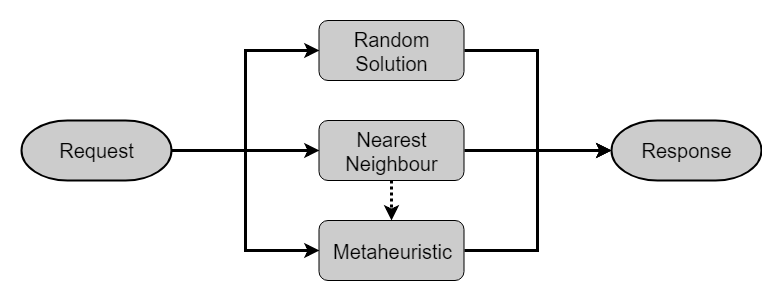
\includegraphics[width=\textwidth]{./Figures/system_design/utility.png}
  \caption{Simplified illustration of the optimization system, which utilizes different algorithms 
  to produce a solution to a user defined request.}
  \label{fig:optimization_system}  
\end{figure}

Having an optimization system which employes multiple, very different, optimization algorithms,
enables the comparison of both the time, and the quality of the proposed solutions.
We known apriori that the random solution is fast, and that its quality is probabily bad.
On the other hand, we expect the more specific algorithms to be slower, but present better solutions.
The goal than to verify if the solution is actually better, how significant the improvement is,
and how much time was necessary to produce such an improvement.



